% Part: biographies 
% Chapter: bertrand-russell
% Section: biography
\documentclass[../../../include/open-logic-section]{subfiles}

\begin{document}

\olfileid{bio}{ber}{bio} 
\olsection{Biography}

\begin{figure}[h!] 
\centering
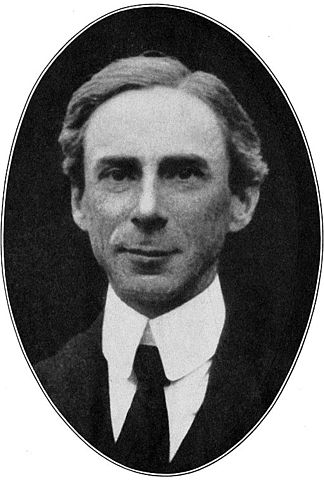
\includegraphics[scale=0.5]{bertrand-russell.jpg} 
\caption{Bertrand Russell. Photo Credit: Wikimedia.} 
\end{figure}
Bertrand Russell is often hailed as one of the founders of analytic philosophy.
Born May 18, 1872, Russell was not only known for his work in philsoophy and logic,
but wrote many popular books in various subject areas. Throughout his life he
was an ardent political activist.
Russell was born in Trellech, Monmouthshire, Wales. His parents were members of 
the British nobility, although they died when he was young, and Russell was sent to 
live with his grandparents, where his upbringing was religious and repressive.

Russell's influence in analytic philosophy, and especially logic, is tremendous. He studied
mathematics and philosophy at Trinity College, Cambridge, where he was influenced by
mathematician Alfred North Whitehead. In 1910, Russell and Whitehead published the
first three volumes of \emph{Principia Mathematica}, where they championed the view
that mathematics is reducible to logic. He then went on to publish major works, such as
his essay \emph{On Denoting}, a book on the theory of types, and many others.
He won the Nobel Prize for literature in 1950.

Russell's life was filled with interesting and idosyncratic events. He was deeply entrenched
in politics and social activism; during World War I he was 
arrested and sent to prison for six months due to pacifist activities. He remained a pacifist
throughout his life, and was again sent to jail for attending a nuclear disarmorment rally 
in 1961. He also survived a plane crash in 1948, where the only survivors were those
sitting in the smoking section. As such, Russell claimed that he owed his life to smoking.
Russell was also known to be a ladies man, and he was married four times, but is said to
have had many extra-marital affairs.

Russel passed away on February 2, 1970 at the age of 97 in Penrhyndeudraeth, Wales.

\end{document}